\clearpage
\item \points{30} {\bf Neural Networks: MNIST image classification}

In this problem, you will implement a simple convolutional neural network
to classify grayscale images of handwritten digits (0 - 9) from
the MNIST dataset. The dataset contains 60,000 training images and
10,000 testing images of handwritten digits, 0 - 9. Each image is
28$\times$28 pixels in size with only a single channel. It also includes labels for each example, a number
indicating the actual digit (0 - 9) handwritten in that image.

The following shows some example images from the MNIST dataset: \footnote{https://commons.wikimedia.org/wiki/File:MnistExamples.png}

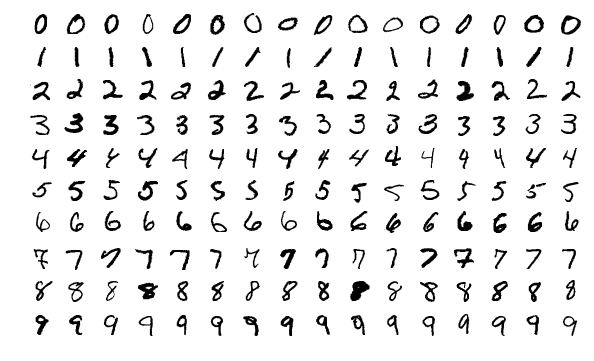
\includegraphics[scale=0.5]{01-nn-mnist/mnist_plot.png} 


The data for this problem can be found in the data folder as \texttt{images\_train.csv}, \texttt{images\_test.csv}, \texttt{labels\_train.csv} and \texttt{labels\_test.csv}.


The code for this assignment can be found within \texttt{p1\_nn.py} within the src folder.

The starter code splits the set
of 60,000 training images and labels into a sets of 59,600 examples as
the training set and 400 examples for dev set.

To start, you will implement a simple convolutional neural network
and cross entropy loss, and train it with the provided data set. 

The architecture is as follows:
\begin{enumerate}

    \item The first layer is a convolutional layer with 2 output channels with a convolution size of 4 by 4.
    \item  The second layer is a max pooling layer of stride and width 5 by 5.
    \item  The third layer is a ReLU activation layer.
    \item  After the four layer, the data is flattened into a single dimension.
    \item  The fith layer is a single linear layer with output size 10 (the number of classes).
    \item  The sixth layer is a softmax layer that computes the probabilities for each class.
    \item  Finally, we use a cross entropy loss as our loss function.
\end{enumerate}

We have provided all of the forward functions for these different layers so there is an unambigious definition of them in the code. Your job in this assignment will be to implement functions that compute the gradients for these layers. However, here is some additional text that might be helpful in understanding the forward functions.

We have discussed convolutional layers on the exam, but as a review, the following equation defines what we mean by a 2d convolution:

\begin{align*}
output[out\_channel, x, y] &=  convolution\_bias[out\_channel] + \\
    & \sum_{di, dj, in\_channel} input[in\_channel, x + di, y + dy] * \\
                   & \qquad \qquad \qquad convolution\_weights[out\_channel, in\_channel, di, dj]
\end{align*}

di and dj iterate through the convolution width and height respectively.

The output of a convolution is of size (\# output channels, input width - convolution width + 1, output height - convolution height + 1).
Note that the dimension of the output is smaller due to padding issues.

Max pooling layers simply take the maximum element over a grid.

It's defined by the following function

$$
output[out\_channel, x, y] = 
    \max_{di, dj} input[in\_channel, x * pool\_width + di, y * pool\_height + dy]
$$

The ReLU (rectified linear unit) is our activation function.
The ReLU is simply $max(0, x)$ where x is the input.

We use cross entropy loss as our loss function. Recall that for a single example $(x, y)$, the cross
entropy loss is:
$$CE(y, \hat{y}) = - \sum_{k=1}^K y_k \log \hat{y_k},$$
where $\hat{y} \in \mathbb{R}^{K}$ is the vector of softmax outputs
from the model for the training example $x$,
and $y \in \mathbb{R}^{K}$ is the ground-truth vector for the training example
$x$ such that $y = [0,...,0,1,0,...,0]^\top$ contains a single 1 at the
position of the correct class (also called a ``one-hot'' representation).

We are also doing mini-batch gradient descent with a batch size of 16. Normally we would iterater over the data multiple times with multiple epochs, but for this assignment we only do 400 batches to save time.

\begin{enumerate}
\item \points{20}

Implement the following functions within \texttt{p1\_nn.py}. We recommend that you start at the top of the list and work your way down:

\begin{enumerate}
\item \texttt{backward\_softmax}
\item \texttt{backward\_relu}
\item \texttt{backward\_log\_loss}
\item \texttt{backward\_linear}
\item \texttt{backward\_convolution} 
\item \texttt{backward\_max\_pool}

\end{enumerate}

\item \points{10}
Now implement a function that computes the full backward pass.

\begin{enumerate}

\item \texttt{backward\_prop}

\end{enumerate}

\end{enumerate}
